This section describes the Balloons Client system in detail and gives
reasoning behind some of the design decisions that were made. The Client system
is the system which the user interacts with on the screen; it makes use of the
Microsoft Kinect hardware to provide natural user input and connects to the 
Balloons Server to manage the items on screen. 

This document only describes the technical aspects of the Client system; for 
design decisions and specification relating to the user interface and input 
controllers please consult the Client Design document.

\subsection{System Design}
As much as is possible, the Client system is split into four components: 
Network, Graphics, Physics and Input; however these four components also need 
to be tied up in a central location --- XNA puts the burden of this into the Game
class. With the exception of Graphics which is part of the Game class, each
sub-system has its own code package and is quite discrete from all the other 
parts, i.e. these components are loosely coupled.

The other main part of the Client system is the model objects --- these represent
some of the main objects in the game. They are not true model objects in the
MVC pattern --- some of the models actually contain drawing logic. This allows
the drawing methods to be moved out of the main graphics system and makes the
system more coherent.

\subsection{Models}
\subsubsection{Bucket}
The bucket model represents a paint bucket which can be used to change the 
decoration of a balloon. A bucket implementation should implement the abstract
Apply To Balloon method to perform the decoration. Two buckets are currently
included in the system: one which changes the colour of the balloon and one 
which changes the overlay. 

\subsubsection{Client Balloon}
The client balloon model represents a balloon as it appears on screen. It 
contains information pertaining to the balloon's dimensions and also a cache of
any textures which have been generated for that balloon (its image or QR code, 
for example). 

\subsubsection{Client Plane}
The client plane model represents a plane as it appears on the screen, as well
as the banner that it carries along with it.

\subsubsection{Content Box}
The content box model is used to define the logic for drawing a content box to
the screen. Two content box implementations are available: one which uses raw
XNA drawing calls to position elements, and one which uses HTML to render the
content. The HTML renderer was a feature added mid-way through development but
is now the default model as it is easier to customize and looks much more
appealing. 

\clearpage{}
\subsection{Network Subsystem}
The Network Subsystem implements the INetworkManager interface and is 
responsible for managing communication between the Client and Server. The 
default implementation relies on the ScreenConnection class from the Messaging
library, details of which can be found elsewhere. 

\begin{table}[H]
\begin{tabular}{|p{4.8cm}|p{3.8cm}|p{7cm}|}
\hline
\multicolumn{3}{|c|}{INetworkManager} \\ \hline
Connect & & Connects the Network Manager to the Server. \\ \hline

MoveBalloonOffscreen & Balloon,\newline Direction,\newline Exit Position,\newline Velocity &
Sends a message to the Server telling it the given balloon has moved off 
screen. The direction is the side the balloon exited, the position a number 
between 0 and 1 of the height of the balloon, and velocity the velocity of the
balloon as it left. \\ \hline

NotifyBalloonPopped & Balloon & 
Sends a message to the Server telling it the given balloon has been popped by
the user. \\ \hline

GetBalloonDetails & Balloon ID &
Retrieves the details of the given balloon from its ID. \\ \hline

UpdateBalloonDetails & Balloon & 
Processes messages from the Server and will be called once per Update loop.
The four parameters are Actions which are called when the relevant message is
received from the Server. \\ \hline

ProcessMessages & On New Balloon,\newline On Pop Balloon,
\newline On Content Update,\newline On State 
Update &
Processes messages from the Server and will be called once per Update loop. 
The four parameters are Actions which are called when the relevant message is
received from the Server. \\ \hline
\end{tabular}

\caption{\emph{INetworkManager} reference}

\label{NetworkManagerRef}
\end{table}

\clearpage{}
\subsection{Physics Subsystem}
The Physics Subsystem is concerned with tracking physical objects in the game
and generates events based on collisions between them. This subsystem is 
slightly more coupled than other classes as it is not coded to an interface; 
this is because the physics and graphics systems are quite interdependent. 
Several methods are available on the Physics Manager to translate from world 
co-ordinates to screen ones. 

During the main loop, the Game System has to feed in the co-ordinates from the
Input system to the Physics system in order for the positions of the hands to 
be updated correctly. The Physics Manager makes use of a class called World
Entity; this class represents an object as it is stored in the world and is 
used by the Game System to track the relationship between physical entities and
model objects.

\begin{longtable}{|p{4.5cm}|p{3.5cm}|p{7.7cm}|}
\caption{\emph{PhysicsManager} reference \label{PhysicsManagerRef}}
\\
\hline
\multicolumn{3}{|c|}{PhysicsManager} \\ \hline

Initialize & Hand Size &
Initialises the Physics Manager. In our system, this creates the Farseer World
object. The Hand Size is provided as it is based on the size of the texture 
loaded in. \\ \hline

Update & Game Time &
Advances the physics world by the specified time. This is called once per call
of the Update method in the Game System.\\ \hline

Create Balloon & Position,\newline Velocity,\newline \emph{Returns} World Entity &
Creates a World Entity object for a balloon. This object will be added to the 
Physics Manager's internal list of Balloons and will cause events to fire when
certain collisions are detected with it.\\ \hline

Create Boundary & Width,\newline Position,\newline \emph{Returns} World Entity &
Creates a physical boundary in the system --- used to create the roof and the 
floor. Currently only horizontal boundaries can be created by this function.
Vertical boundaries are not handled by the physics engine but by the Game (as 
they fire network events).\\ \hline

Update Hand Positions & Array of Hands &
Updates the positions of the hands in the system. If a Hand object passed in 
is not currently tracked by the system, a new World Entity is created for it.
\\ \hline

Get Hand Positions & \emph{Returns} List of World Entity &
Returns the World Entity object for each hand currently tracked by the system.
\\ \hline

Get Hand For Entity & World Entity,\newline \emph{Returns} Hand &
Returns the Hand object for the World Entity provided. Used by the Game System
to draw the hand on screen. \\ \hline

Enable Handle Collisions & &
Enables collisions between hands and balloons. \\ \hline

Disable Hand Collisions & &
Disables collisions between hands and balloons. Used when the content box is 
up to avoid the weird feeling of colliding with balloons that the user can't 
see. \\ \hline

Apply Wind & & 
Applies a force to all the balloons to simulate wind. \\ \hline

Remove Entity & World Entity &
Removes the given entity from the physics world. Hand entities are not removed
with this function and would be regenerated on the next call to Update Hand 
Positions anyway. \\ \hline

\emph{Static} World To Pixel & World Position\newline \emph{Returns} Screen Position &
Converts a physics world co-ordinate to a screen co-ordinate.\\ \hline

\emph{Static} Pixel To World & Screen Position\newline \emph{Returns} World Position &
Converts a screen co-ordinate to a physics world one.\\ \hline

\emph{Static} World Body To Pixel & World Position,\newline Pixel Offset,\newline 
\emph{Returns} Screen Position &
Converts a physics world co-ordinate to a screen co-ordinate, minus a pixel 
offset (usually the width of a texture).\\ \hline

\emph{Static} Pixel To World Body & Screen Position,\newline Pixel Offset,\newline
\emph{Returns} World Position & 
As World Body to Pixel but in reverse.\\ \hline

\emph{Event} Balloon Popped & BalloonPopped\-EventArgs &
Fired when the Physics Manager detects that a user has popped a balloon.
\\ \hline

\emph{Event} Bucket Collision & BucketCollision\-EventArgs & 
Fired when the Physics Manager detects that a balloon has collided with a 
bucket.\\ \hline

\end{longtable}

\clearpage{}
\subsection{Input Subsystem}
The Input Subsystem tracks user input and is defined by the IInputManager
interface (see table \ref{InputManagerRef}. Two input subsystems are implemented in 
the project: one for using the Kinect, and one for using the Mouse. The Kinect 
system is described elsewhere in this report; the Mouse system is very simple in 
comparison.
 
When no mouse buttons are pressed, the mouse emulates a single hand which is
centred on the position of the mouse. If the left mouse button is held down, a
second hand appears with its position relative to the first hand. If, whilst
still the left mouse button is still down, the right mouse button is also
depressed, then the two hands will emulate a clapping motion.

\begin{table}[H]
\begin{tabular}{|p{3.6cm}|p{3cm}|p{9cm}|}
\hline
\multicolumn{3}{|c|}{IInputManager} \\ \hline
Initialize & Screen Size & 
Initialises the Input Manager. Some Input Devices use normalised dimensions so
the screen size parameter should be stored as the values returned by this 
Interface should be in screen co-ordinates. \\ \hline

GetHandPositions & \emph{Returns} Hand[] &
Returns an array of Hand objects, one Hand per physical hand. A Hand object
describes the position of a single hand and has an identifier to tell which
user the hand belongs to. 
The Hand objects must be static between calls; i.e. a Hand object should
represent a physical hand for the duration of said hand being focused as an
input entity. If this is not the case, and a new Hand object is generated 
every frame, the physics engine will not work correctly. \\ \hline
\end{tabular}
\caption{\emph{IInputManager} reference}

\label{InputManagerRef}
\end{table}

\subsection{Graphics \& Game Systems}
The main logic for the Graphics Subsystem lies in the Game System itself. XNA
defines a layout for the Game System, in which game logic should be performed
in the Update method and drawing logic in the Draw method (see table
\vref{BalloonClientRef}). The Game System also
ties together all the other components.

\begin{table}
\begin{tabular}{|p{3cm}|p{3.6cm}|p{9cm}|}
\hline
\multicolumn{3}{|c|}{BalloonClient} \\ \hline
\emph{Constructor} & Network Manager, Input Manager & 
Creates a new instance of the Balloon Client using the provided Network and 
Input Managers. (These are injected from the main method which determines which
to use from the Configuration object). This constructor also creates the 
Graphics Device Manager used by XNA and initialises the Input Manager with the
screen dimensions. \\ \hline

Load Content & & 
This is a method called by XNA and is used to load external content. It creates
a new Sprite Batch, loads in fonts and textures, and sets up the mappings so we
can access the textures quickly and easily in code. \\ \hline

Initialize & &
Initialize sets up the Physics Manager and the collision detection handlers, 
then creates the roof and floor boundaries. It creates the buckets using a 
formula to determine the gap between them. Finally, it asks the Network Manager
to connect to the server. \\ \hline

Update & Game Time &
Update performs the game logic. The following steps are performed:
\begin{itemize}
	\item{Process Network Events}
	\item{Process Input}
	\item{Process Physics (and Apply Wind)}
	\item{Move any balloons to other screens which have moved off the edge of the screen}
	\item{Update any running animations}
	\item{Update the content box (if it is visible)}
\end{itemize}
\\ \hline

Draw & Game Time &
Draw performs the actual drawing of the game world. It is not supposed to 
perform any logic tasks. Items drawn first will be hidden ``behind'' items drawn
later. The following steps are performed:
\begin{itemize}
	\item{Clear the screen and initialise the Sprite Batch}
	\item{Draw the background}
	\item{Draw the balloon captions}
	\item{Draw the balloons}
	\item{Draw the ``pop'' animations}
	\item{Draw the buckets}
	\item{Draw the content box (if it is supposed to be visible)}
	\item{Draw the user's hands}
	\item{Flush the Sprite Batch}
\end{itemize}
\\ \hline
\end{tabular}
\caption{\emph{BalloonClient} reference}

\label{BalloonClientRef}
\end{table}

\clearpage{}
\subsection{Development Report}
Throughout the development cycle of the project, several builds were presented
to the client. In the first few weeks, many of the demo builds were individual
feasibility studies of individual components needed to build the final project.
This section gives details of what requirements were implemented in the Client
system for each week.

\subsubsection{Client Demo 1 - 7th February}
\begin{figure}[h]
\begin{centering}
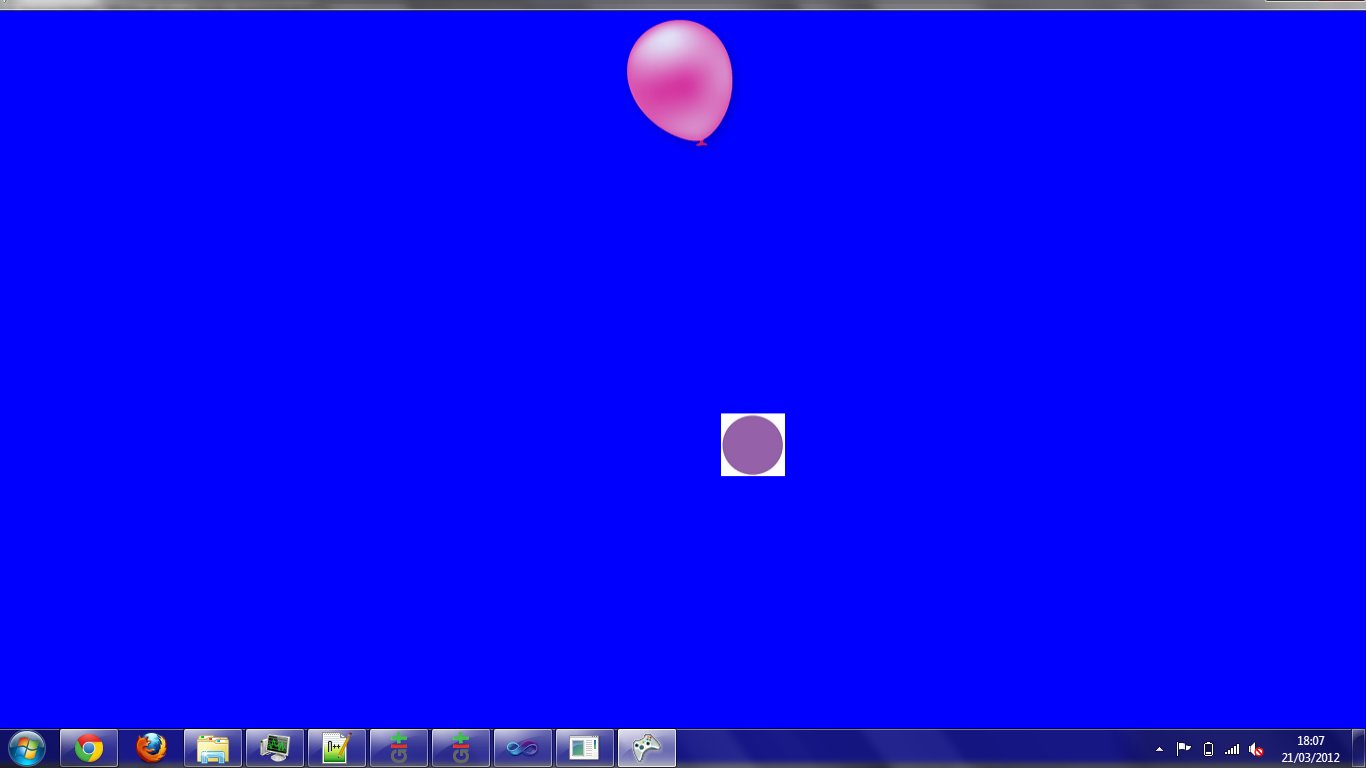
\includegraphics[width=\textwidth]{Diagrams/Client-Log-W4.jpg}
\par\end{centering}

\caption{Prototype in Week 4}
\end{figure}
The first prototype presented to the client showed hand tracking using the
Kinect and the capabilities of the physics engine using mock graphics. The
client thought that the Kinect input seemed to work well and was generally
pleased with the input at this stage.

Another prototype build during this week's meeting demonstrated the design of
the user interface which the user was also pleased with; however that prototype
was discarded as it was easier to implement the design on top of the input
prototype.

\subsubsection{Client Demo 2 - 14th February}
\begin{figure}[h]
\begin{centering}
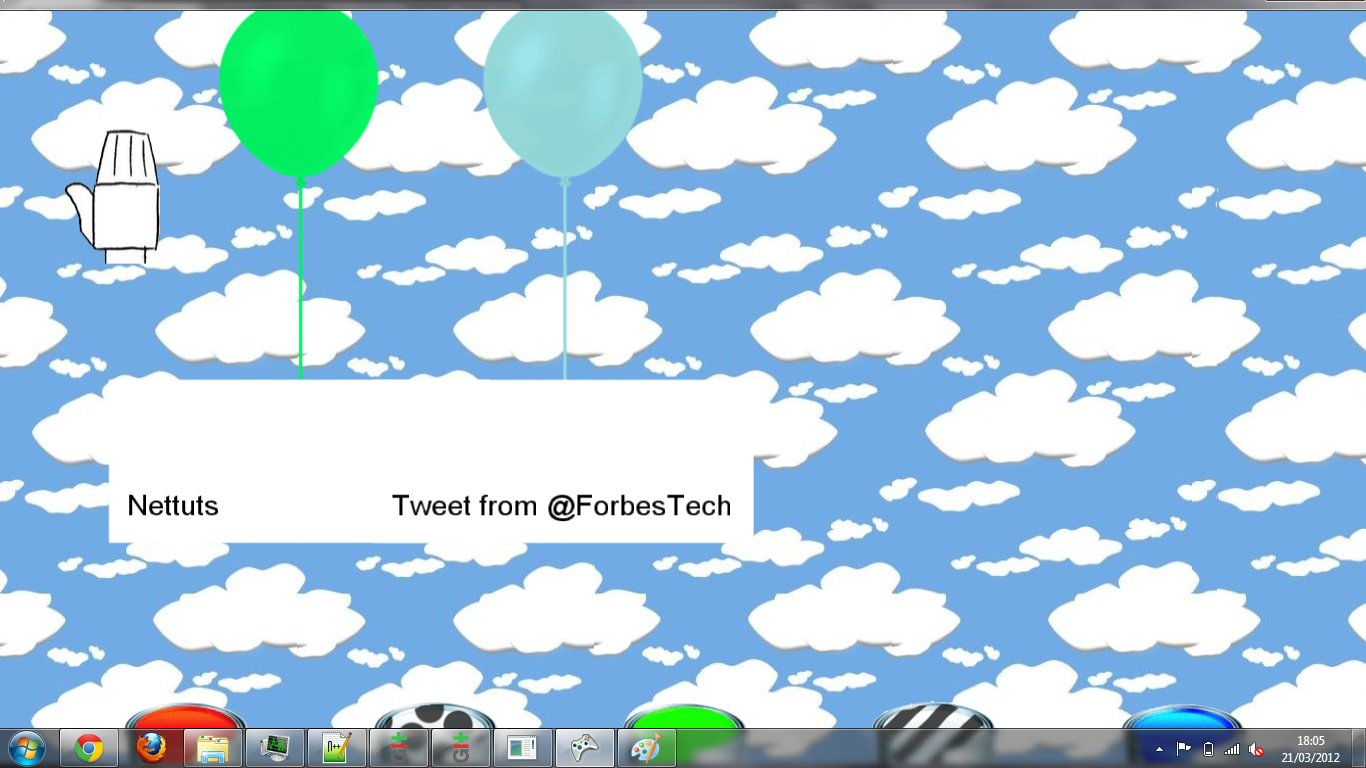
\includegraphics[width=\textwidth]{Diagrams/Client-Log-W5.jpg}
\par\end{centering}

\caption{Prototype in Week 5}
\end{figure}
The second demo prototype was much more advanced than the first. Many of the UI
concepts were implemented including balloons along with buckets to provide the 
``painting'' functionality. The mock graphics used in the first prototype were 
replaced by nicer images. The balloons were already tied into the physics 
however the rules were tweaked to make them much more realistic. The ability to
view the content of a balloon was also added by putting in a ``pop balloon'' 
action in the Input interface, which when called, caused a content box to open
with the desired content. Balloons were also given a small ``tag'' with a short
text description.

The Kinect input system was now governed by the physics engine. Whilst this 
allowed for collision detection, the user input lag added caused the client 
some issues as it ran very slowly on the target hardware. Furthermore, the
client had issues reaching the top of the screen on the target hardware.

Finally, the networking features of the system were added in this build. These
allowed balloons to be generated by the Server and pushed down to the Client 
system. Balloons could be pushed between screens, however bugs in the 
server made this difficult to demonstrate.

\subsubsection{Client Demo 3 - 21st February}
\begin{figure}[p]
\begin{centering}
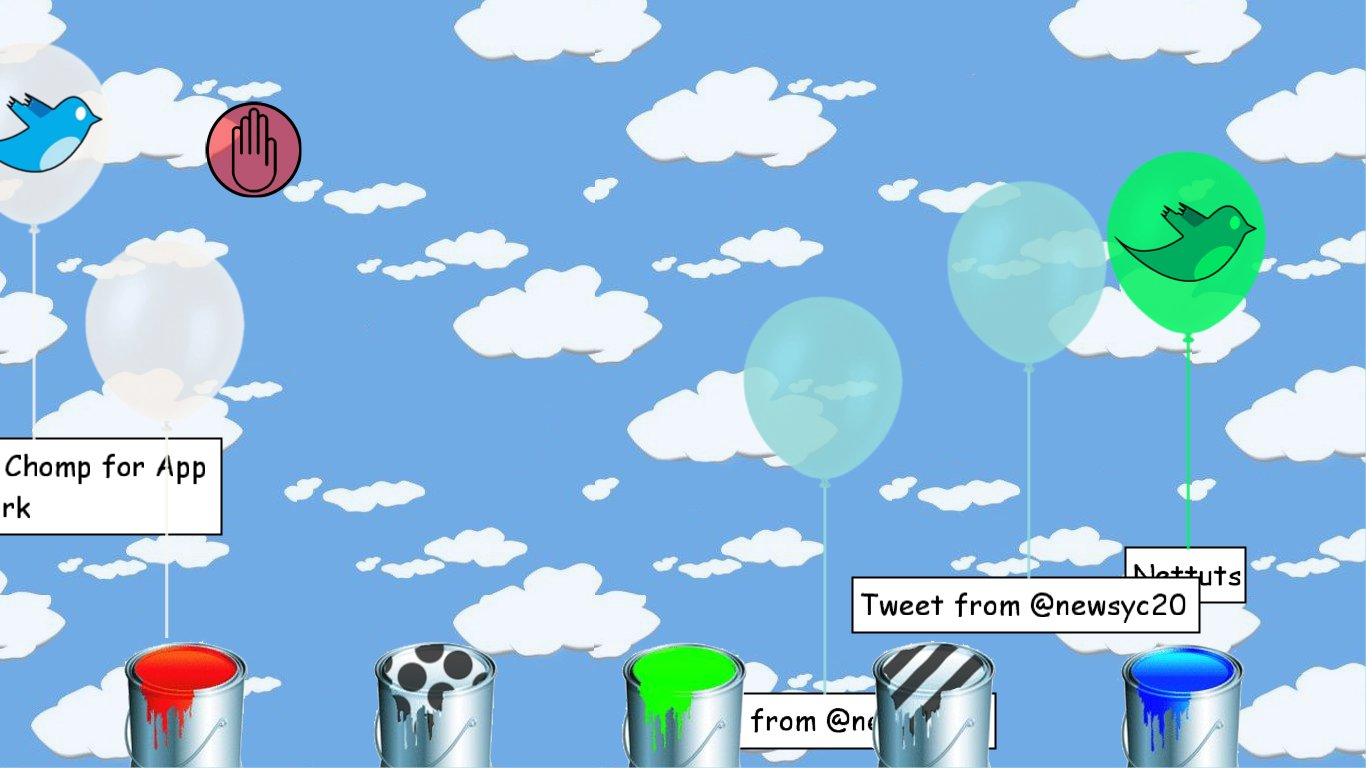
\includegraphics[width=\textwidth]{Diagrams/Client-Log-W6-XNA.jpg}
\par\end{centering}

\caption{Prototype in Week 6 Using XNA Labels}
\end{figure}
\begin{figure}[p]
\begin{centering}
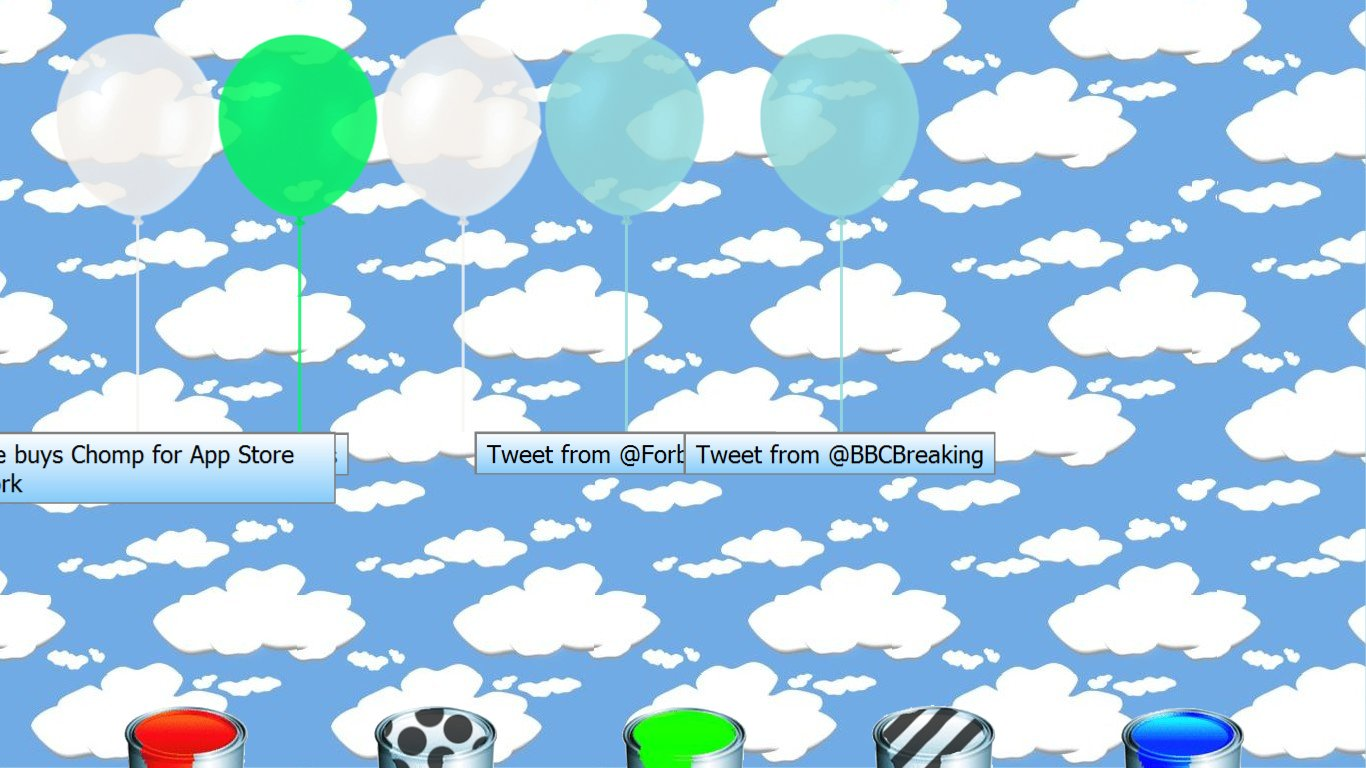
\includegraphics[width=\textwidth]{Diagrams/Client-Log-W6-HTML.jpg}
\par\end{centering}

\caption{Prototype in Week 6 Using HTML Labels}
\end{figure}
Several bug fixes and improvements were implemented for this build. Crashes 
from the previous build were ironed out and fixed; the issue with the user 
being unable to reach the top of the screen was also fixed. Text-wrapping on 
the balloon tags was fixed and the tag boxes made to fit the text once it had
been wrapped to remove any extra white space.

The content box was improved and made to show images and a QR Code which 
encoded the URL of the content article, allowing a user to visit that link with
a mobile device. A timer was added to the content box showing the user how long
until it automatically closed and a large button was placed in the top right of
the screen which the user could use to close the box themselves. An HTML 
version of the content box was also implemented, it was planned to replace the
hard coded versions in the final release. 

Overall the client was very pleased with the improvements made to the system.
Unfortunately it seemed impossible that the Client System could be run on the
target hardware; this demo was shown using a laptop hooked up to the screens
rather than the hardware.

\subsubsection{User Evaluation Build - 27th February}
During the user evaluation some fixes were applied to prevent concurrency 
issues in the HTML renderer when rendering images; other than this the Client 
system's build was unchanged from the previous week.

\subsubsection{User Evaluation Iteration - 13th March}
\begin{figure}[h]
\begin{centering}
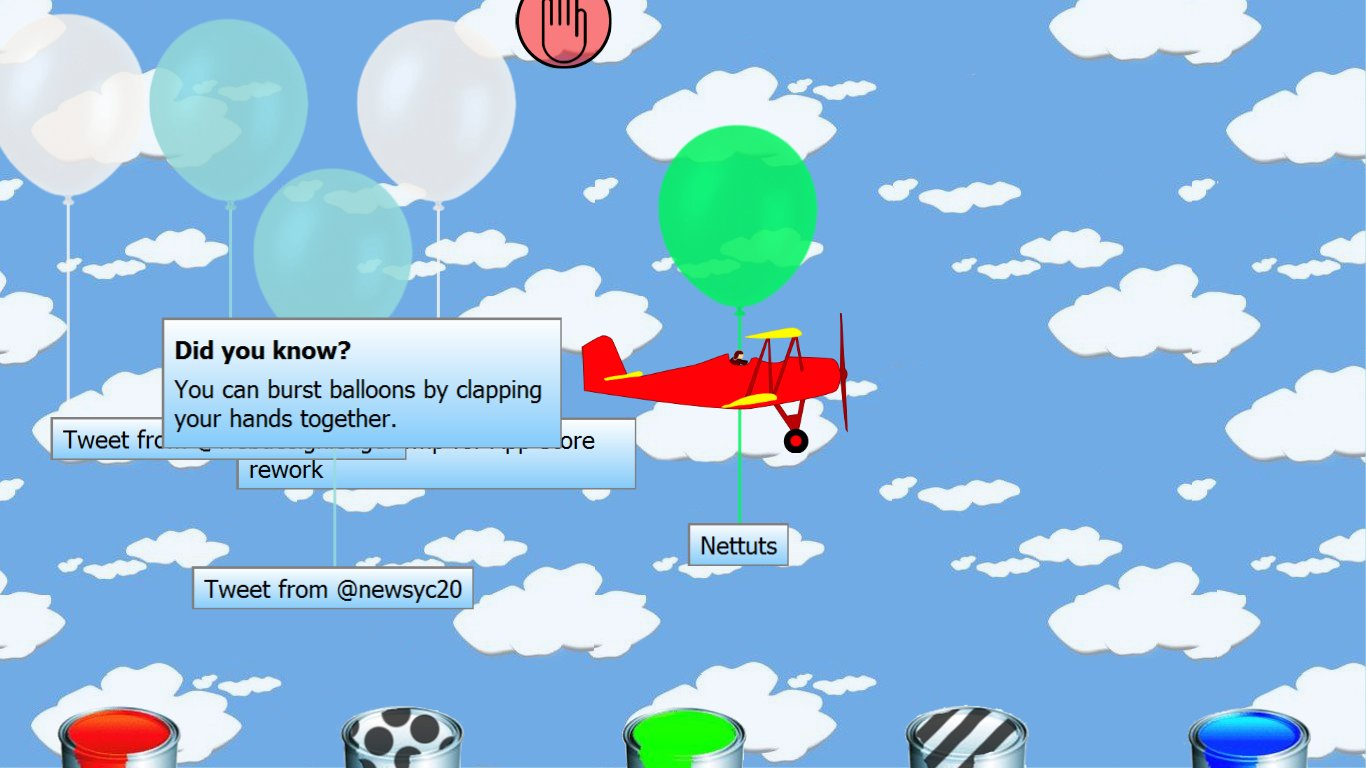
\includegraphics[width=\textwidth]{Diagrams/Client-Log-W10.jpg}
\par\end{centering}

\caption{Final Product}
\end{figure}
From the results of the user evaluation we implemented several fixes to do with
usability --- these included:
\begin{itemize}
\item{Tweaks to the close button for the content box which users found clunky 
to use. We added a black border to it, reduced the activation time from 2.5s to
0.5s and added a second close button in the top-left.}
\item{Paint buckets were too close together; they were spaced out slightly 
further.}
\item{The physical floor was raised slightly whilst moving the buckets down. 
This prevents balloons from being ``stuck'' under the floor.}
\item{Animations were added after a period of inactivity which inform the user
of actions they can take to interact with the system.}
\end{itemize}

\clearpage{}

\subsection{Third-Party Components}
The Client system makes use of several third-party components to reduce the 
amount of development required:

\begin{itemize}
\item{Microsoft XNA Game Studio 4.0}

An environment for quickly creating games which provides several library 
functions such as loading content and drawing to the screen. 
\item{Microsoft Kinect SDK 1.0}

The official SDK providing the ability to interact with the Kinect hardware. 
\item{Farseer Physics 3.3}

A physics library derived from Box2D, a very popular physics library on which
many iPhone and Android games are based. It is used to provide collision 
detection and object interaction between balloons and gives a realistic feel to
balloon movement.
\item{Terra Informatica HTMLayout}

A lightweight HTML renderer used to render the labels and content boxes of 
balloons. This allowed us to provide much richer content than the built-in text
rendering abilities of XNA.
\item{ThoughtWorks QRCode}

A QRCode generation library, used to convert content URLs into a format which 
can be quickly recognised by a user's device.
\end{itemize}
